\section{Introduction}
\label{introduction}
%\begin{itemize}
	%\item What are Cyber-Physical Systems?
    %\item What are the unique challenges of developing CPS compared to other systems?
    %\item How to guarantee the safety of CPS?
    %\item What is the current practice?
    %\item What is the difference between requirements and specifications?
    %\item What is closed-loop verification? Is it necessary?
    %\item What is model-based design? What are the benefits and limitations?
    %\item What are the different techniques of model-based closed-loop verification? 
    %\item In which steps during the software life cycle are those techniques used?
    %\item What is model checking? What guarantee can it provide? What are the challenges?
    %\item What are the focus difference between environment modeling and system modeling, in general and in each step?
    %\item What is model abstraction/approximation? What information are lost during this process?
    %\item How to keep track of these information? Where can they be used?
    %\item What is over-approximation? What are the limits?
    %\item What is the appropriate model complexity?
    %\item What aspects affect the required model complexity?
    %\item How to manage complexity for the system model?
    %\item Why CEGAR cannot be applied to the environment model?
    %\item How to manage the complexity of the environment model?
    %\item What are domain knowledge? Where have we used them?
    %\item How can we encode domain knowledge used during model development and abstraction?
    %\item Can we use encoded domain knowledge to manage complexity of the environment model? How?
    %\item The case study on heart model and pacemaker sounds good. Is the approach general enough?
%\end{itemize}

Implantable medical devices like pacemakers are designed to improve certain undesired physiological conditions with very little human interventions. Their capability of autonomously affecting the physiological conditions of the patients makes the medical devices safety-critical, and sufficient evidence on the safety and efficacy of the devices should be provided before the devices can be implanted in the patients. As more functions added to the devices, the complexity of the software component of the device is increasing dramatically, leading to more and more potential safety violations due to software bugs. To ensure the safety of medical device software, the device software not only have to conform with its design, which is specified in \emph{Software Specifications}

\subsection{Challenges}
In this paper, we address the following four challenges that stand in the way of applying formal methods to the problem of verifying the correct functioning of pacemakers and other implantable cardiac devices.

\begin{enumerate}
	\item There are no formal models of the human heart's behavior.
	\item There is a wide variety of distinct heart conditions, many of which are ill- or incompletely understood.
	This results in the a priori need to create many heart models.
	\item The physiological requirements are worded in the language of physicians and medical practicionners, so there is a need to express these requirements formally.
	\item A related challenge is that these requirements are often vague, in the sense that a violation of the requirement does not necessarily indicate a preventable issue or a bug in the pacemaker. 
	Thus there is a need to transmit back our findings to the physicians and device manufacturers who can decide whether the found counter-example is a bug or not.
\end{enumerate}

\textcolor{red}{Question to be resolved: why is the application of abstraction rules preferred to `regular' predicate-based abstraction?
 }
\subsection{The Model Checking Problem}
%Model-based design enables closed-loop verification at an early design stage. 
For a model $M$ with state space $S$, we define the behavior of the model as an execution trace in $\delta\in S^*$. The reachable behavior space of model $M$ is denoted as $\mathbb{B}(M)\subset S^*$. A property $\varphi$ defines a region in the behavior space within which the property is satisfied, which can be denoted as $\mathbb{B}(\varphi)$. A model checking problem is to use mathematical tool to explore the whole reachable behaviors of a model $M$ against a property $\varphi$ such that $\mathbb{B}(M)\subseteq \mathbb{B}(\varphi)$. We denote it as $M\models\varphi$. Property violations should be returned as execution traces $\delta_v$ so that the designer can analyze and address the problem. 

\subsection{Model Abstraction with Over-approximation}
The behavior space of the actual system is too large for model checker to exhaustively explore. A model of the system which covers all behaviors of the system can be developed which can not only reduce complexity, but also having the suitable formalism for the model checker. An abstraction function $h$ abstracting model $M$ to $M'$ is a non-surjective function from state space $S$ to the new abstract state space $S'$ such that: 
$$\forall s\in S, \exists s'\in S' \text{ s.t. } h(s)=s'$$
This definition can be extended to behaviors $\delta\in \mathbb{B}(M)$, such that:
$$\forall \delta\in \mathbb{B}(M),\exists \delta'\in\mathbb{B}(M')\text{ s.t. } h(\delta)=h(\delta')$$
From the definition, we know that the abstract model $M'$ covers all behaviors of $M$, which is referred to as \emph{over-approximation}. We represent the over-approximation relationship as $M'\models M$, and the relationship between reachable behavior spaces as $\mathbb{B}(M)\subset_a\mathbb{B}(M')$. Then we have:
$$\mathbb{B}(M')\subseteq_a \mathbb{B}(M),\mathbb{B}(M)\subseteq_a \mathbb{B}(\varphi)\rightarrow\mathbb{B}(M')\subseteq_a \mathbb{B}(\varphi)\rightarrow M_t\models\varphi$$
Since the properties are preserved In general the state space of $S'$ is smaller than $S$ while still preserve the property, during model checking the more abstract model can be used to check the property. 

\subsubsection{Context Ambiguities}
Since $h$ is non-surjective, certain states in $S$ will not be distinguishable in $S'$:
$$\exists s_1,s_2\in S \text{ s.t. }h(s_1)=h(s_2)=s',s'\in S'$$
For behaviors we have:
$$\exists \delta_1,\delta_2\in \mathbb{B}(M) \text{ s.t. }h(\delta_1)=h(\delta_2)=\delta',\delta'\in \mathbb{B}(M')$$
In the abstract model $\delta_1$ and $\delta_2$ are not distinguishable
\subsubsection{Validity Ambiguities}
However since $h$ is non-surjective, there exists behaviors in $M'$ that do not exists in the original model $M$:
$$\exists\delta'\in\mathbb{B}(M')\text{ s.t. }h^{-1}(\delta')\not\subset\mathbb{B}(M)$$

\subsubsection{System Model vs. Environment Model}
\subsection{Closed-loop Model Checking}
%During the software development process, there are two key documents that track the safety and efficacy of the software component, namely the \textbf{Software Requirements} and \textbf{Software Specifications}. These two terms are sometimes used interchangeably, however, requirements and specifications provides different angle of system safety and require very different verification techniques.
%
%A requirement states the objective of the system in design in terms of environmental conditions. For example, a requirement of a self-driving car would be: \emph{The car should not hit a pedestrian.} A specification is how the system developers propose to satisfy the requirements. For example, the specification corresponding to the requirement of a self-driving car would be: \emph{If an object is detected in front of the car and the distance to the object is less than $d$, the car should brake.} As we can see, a specification may not satisfy the corresponding requirement, thus two steps are required to guarantee the safety of the system software. The first is the conformance between the system software and the software specification. The second one is whether the software specifications can satisfy all the software requirements.
%
%Currently in most system design, the conformance between the software specifications and the system software are verified using extensive \textbf{open-loop} testing. The test cases are extracted from the system software using static analysis based on certain coverage criteria. The conformance between the specifications and the requirements are maintained by traceability documents, which is insufficient for safety guarantee.
% \begin{figure}[!t]
% 		\centering
% 		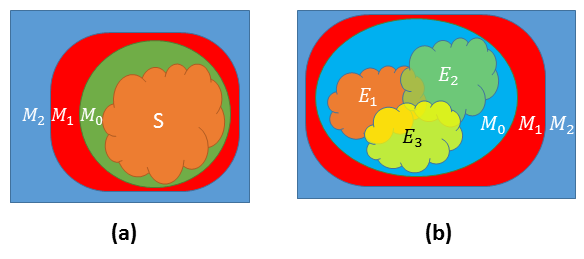
\includegraphics[width=0.8\textwidth]{figs/SysVSEnv.png}
% 		%\vspace{-5pt}
% 		\caption{\small Modeling in terms of behavior coverage. As model becomes more abstract, the coverage increases while the boundary becomes more simple. (a) System modeling in which there is only one concrete system; (b) Environment modeling in which abstraction can be used to generalize different conditions}
% 		  %\vspace{-15pt}
% 		\label{fig:sys}
% \end{figure}
\begin{figure}[!t]
		\centering
		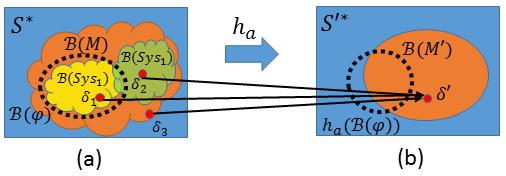
\includegraphics[width=0.8\textwidth]{figs/distinction.png}
		%\vspace{-5pt}
		\caption{\small }
		  %\vspace{-15pt}
		\label{fig:ambiguity}
\end{figure}
\begin{figure}[!t]
		\centering
		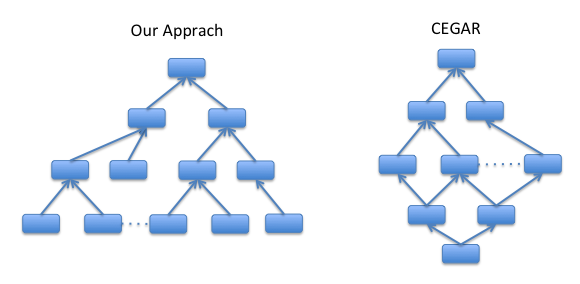
\includegraphics[width=0.8\textwidth]{figs/env_sys.png}
		%\vspace{-5pt}
		\caption{\small }
		  %\vspace{-15pt}
		\label{fig:distinction}
\end{figure}

Since the requirements describe the intended behaviors of the closed-loop system consists of the environment and the system, verifying whether the specifications of the system satisfy the requirements requires closed-loop verification. In the medical device industry, closed-loop verification is performed in the form of clinical trials in which the devices are tested on the real patients. Clinical trials can only cover very limited environmental conditions due to extremely high cost. Moreover, clinical trials are often conducted at the last design stage. Fixing bugs at this stage is also very costly.

Model-based design has been proposed to speed up system software design and provide sufficient safety maintaining the safety promises in software requirement. It can potentially enable closed-loop verification of the software requirements at an earlier stage thus reduce cost. In a model-based design framework, the system software is first designed as an abstract model. Together with an environment model the closed-loop system can be verified against software requirements using model-checking techniques. The verified system model can then be rigorously translated into the software implementation (semi-)automatically so that the software implementation also satisfies all the software requirements.

%The software and its environment have very different properties that modeling them requires very different focuses. The software is generally a control graph which is generally deterministic given with physics and computations are two different things.

One of the biggest challenge for model-based design is to manage how much detail a model should have during model checking. In general the model should be abstract enough to ignore unnecessary details in order to reduce computational cost, but also detailed enough to distinguish execution paths that 1) satisfy/violate a property, and/or 2) are valid/invalid due to the extra behaviors introduced during model abstraction/approximation. These ambiguities must be removed from model to prevent false positives/negatives during model checking. 

\subsection{Outline of the paper}
\begin{itemize}
	\item Section 2: Basic state space formulation with transition groups
    \item Section 3: Formulation of over-approximation and its effect on transition groups
    \item Section 4: Linking transition groups to environmental conditions and thus requirement
    \item Section 5: Rule-based EP heart model abstraction with transition groups
    \item Section 6: Case 1: Requirement-guided model refinement during ELT case 
    \item\textcolor{red}{ Section 7: Case 2: Model refinement for eliminating potential ambiguity. With mode-switch case.} 
\end{itemize}

%\section{Closed-loop Model Checking}
%We first define the behavior space of a model as all combinations of states valuations. For a model $M$ with $n$ state variables $v_1\dots v_n$, and each state variable can take value within the domain $D(v_i)$, the size of the overall behavior space is $\Pi_{i=1}^n D(v_i)$. The actual reachable behavior space of a model $M$ is far less and can be defined by $\mathbb{B}(M)$. As a reference or ground truth for behavior space, we assume the behavior space $\mathbb{B}(S)$ for a physical system $S$ which is infinitely large. All the behavior spaces correspond to the models $\mathbb{B}(M)$ of the system are projections from $\mathbb{B}(S)$.  
%\Hao{}
For a model $M$ with state space $S$, we define the behavior of the system as an execution trace in $\delta\in S^*$. The reachable behavior space of model $M$ is denoted as $\mathbb{B}(M)\subset S^*$. For reference we can represent an actual system as a model $M_t$ with infinite details. A property defines a region in the behavior space within which the property is satisfied. The satisfaction region of a property $\varphi$ can be denoted as $\mathbb{B}(\varphi)$. A system $M_t$ satisfies a property $\varphi$ if $\mathbb{B}(M_t)\subseteq \mathbb{B}(\varphi)$. We denote it as $M_t\models\varphi$. 

Models can be abstracted to potentially reduce complexity and increase coverage. An abstraction function $h$ abstracting model $M$ to $M'$ is a non-surjective function from state space $S$ to the new abstract state space $S'$ such that 
$$\forall s\in S, \exists s'\in S' \text{ s.t. } h(s)=s'$$
For a behavior $\delta\in \mathbb{B}(M)$
$$\forall \delta\in \mathbb{B}(M),\exists \delta\in\mathbb{B}(M')\text{ s.t. } h(\delta)=h(\delta')$$
The abstract model $M'$ covers all behaviors of $M$, which is referred to as \emph{over-approximation}. 
As we can see, if $M$ is an over-approximation of $M_t$, meaning $\mathbb{B}(M_t)\subseteq \mathbb{B}(M)$, and $\mathbb{B}(M)\subseteq \mathbb{B}(\varphi)$, we have:
 $$\mathbb{B}(M_t)\subseteq \mathbb{B}(\varphi)\rightarrow M_t\models\varphi$$ 
Since the state space of $S'$ is smaller than $S$ while still preserve the property, during model checking the more abstract model can be used to check the property. 

Since $h$ is non-surjective, 

%No models of the system can match the region of the system exactly due to lack of information. As the model becomes more abstract, the boundary defining the behavior region becomes less complex. If the abstract model covers all the system behaviors such that $\mathbb{B}(S)\subset\mathbb{B}(M)$, the model is referred to as an \emph{over-approximation} of the system. For environment model, over-approximation can also be used to \emph{generalize} different environmental conditions, i.e. in \figref{distinction}.(a) two system behaviors $\mathbb{B}(S_1)$ and $\mathbb{B}(S_2)$ are covered by a model $\mathbb{B}(M)$.


In most of the cases, the internal states and transitions of a system cannot be fully observable. The behavior space can thus be mapped to other observable behavior spaces with less dimensions.
\Hao{Need to clarify/visualize the notion of observability here} 
Note that the observability does not refer to the interface of the system, there can be multiple observable behavior spaces that correspond to different abstraction of the system. As the result, behaviors that are distinguishable in the full behavior space can be indistinguishable in a observable behavior space, causing ambiguities that can result in false-negatives and false-positives during verification. We denote one observable behavior space as $\mathbb{B}_o(S)$. 

As shown in \figref{distinction}, $\mathbb{B}(M)$ and $\mathbb{B}(\varphi)$ are mapped to $\mathbb{B}_o(M')$ and $\mathbb{B}_o(\varphi')$. Three behaviors in $b_1,b_2,b_3\in\mathbb{B}$ are mapped to a single behavior $b'\in\mathbb{B}_o$. Since $b'\not\in\mathbb{B}_o(\varphi')$, it may be returned by verification tools like model checker as counter-example. In $\mathbb{B}_o$ is possible that two categories of ambiguities exist, namely \textbf{Validity ambiguity} and \textbf{Context ambiguity}. %Failure to distinguish these behaviors can cause false-negatives and/or false-positives during verification.

Validity ambiguity refers to the incapability to distinguish a physically possible execution with an invalid one. In \figref{distinction}.(a), $b_3$ is an invalid behavior since it does not belong to either $S_1$ or $S_2$ but it is covered by the model $M$. 

A model $M$ is compatible with an observable behavior space $\mathbb{S}^o$ if all the behaviors that can be generated by $M$ 

A model is appropriate for a property if all its behaviors  



A Counter-Example-Guided Abstraction and Refinement approach has been proposed to automatically derive model with appropriate amount of details. (\cite{CEGAR}) Assume we would like to check the system $S$ against the property $\varphi$. First, the most abstract model $M_0\models^a S$ is derived from the actual system $S$ based on certain abstraction rules, so that it can distinguish all execution paths that satisfy/violate $\varphi$. Then $M_0$ is verified against the property in an automated model checker. If the property is violated $M_0\not\models\varphi$, a counter-example $\delta^c$ is returned by the model checker. $\delta^c$ has to be then validated so that it can be produced by $S$. If the system can produce $\delta^c$, which can be denoted as $\delta^c\triangleleft S$, $\delta^c$ is a valid counter-example. Otherwise $\delta^c$ is regarded as \textbf{spurious} and the model has to be refined so that the $\delta^c$ is not producible by the model. The refined model $M_1\models^a M_0$ is derived by adding back the minimum amount of abstracted details that prevent $\delta^c$ from being enabled, so that $\delta^c\not\triangleleft M_1$. This process continues until either no counter-example is returned, or a counter-example is not spurious. 

CEGAR works very well during system modeling in which there is only one concrete system implementation $S$. However, for closed-loop verification the objective is to check whether $E||S\models\varphi$. If the environment $E$ is also represented by a model during model checking, both $M^E$ and $M^S$ have to be unambiguous. When verifying system specifications, normally there is no constraints on the environment so that there is no spurious counter-examples due to the environment model. In this case CEGAR still works. However in the software requirements, there are constraints on the environment conditions. If these constraints are not enforced in $M^E$, the verification can yield spurious counter-examples. However, CEGAR will not work for environment modeling due to the differences between the environment and the system. In system modeling, there is only one concrete implementation $S$, so if a counter-example $\delta^c$ is returned during model checking, only $\delta^c\triangleleft S$ has to be checked. However, for the environment, there are infinite number of environmental conditions $E_i$, like different patients in the medical device domain. Details are ignored in the abstract models not only to reduce complexity, but also to \textbf{generalize} different conditions so that:
$$\forall \delta\triangleleft E_i, i\in [1,n],\delta\triangleleft M^E$$
Note that during the generalization process, more behaviors of the environment will be introduced into the model: 
$$\exists\delta^s\triangleleft M^E \text{ s.t. } \delta^s\not\triangleleft E_i, i\in [1,n]$$
In this case, if an execution path $\delta$ is returned as a counter-example during model checking on software requirement, there is no way to check whether 
$$\exists i\in[1,n],\delta\triangleleft E_i$$ 
as $n$ may be a large number or is unclear in the first place. As a result, the validity of the counter-example cannot be validated, and therefore the model cannot be refined by analyzing the spurious counter-example. CEGAR is not effective during environment modeling.

In Cyber-Physical Systems, there are \textbf{domain experts} who understand how the environment of the system works. The \textbf{domain knowledge} is a set of environmental constraints which can be used to define different environment conditions, and determine the validity of the execution paths. However, domain knowledge are in general not formalized thus cannot be used in any automated processes. In this paper, we use closed-loop model checking on an implantable pacemaker model as example to demonstrate abstraction and refinement of the environment models using encoding domain knowledge. We use two case studies to demonstrate that although CEGAR is not applicable to the environment model, the domain knowledge can still be used to validate executions and provide potential validity violations.\Hao{Still need to formalize}

The contribution of this paper is two-folds: 1) we formally specified the potential ambiguities during model abstraction and identified the difference between environment modeling and system modeling. 2) We demonstrated the potential application of encoded domain knowledge to eliminate the ambiguities during abstraction and refinement of environment models.
\begin{itemize}
	\item Abstraction rules for environment models 
    \item Appropriate abstraction function check, definition clear, assumptions implicit, especially for environment models
\end{itemize}
%\section{A Simple Example}
Imaging we are developing a high-level control algorithm for an autonomous vehicle
\textsf{A[] (not CarCross $\&\&$ PedCross)}\\
\textsf{E<> (CarCross)}
\begin{figure}[!t]
		\centering
		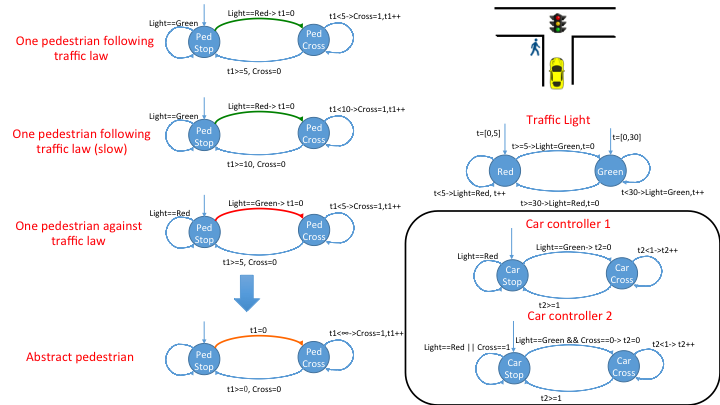
\includegraphics[width=0.9\textwidth]{figs/example.png}
		%\vspace{-5pt}
		\caption{\small }
		  %\vspace{-15pt}
		\label{fig:example}
\end{figure}